\section{Punto de Vista de Implementación y Despliegue}

El punto de vista de la implementación y el despliegue muestra cómo se realizan una o más aplicaciones en la infraestructura. Esto comprende la asignación de las aplicaciones y componentes a los artefactos, y la asignación de la información utilizada por esas aplicaciones y componentes a la infraestructura de almacenamiento subyacente.\\

Un artefacto representa un dato que se utiliza o se produce en un proceso de desarrollo de software, o por el despliegue y funcionamiento de un sistema informático. Un artefacto representa un elemento tangible en el mundo de la informática. El artefacto es una especialización del objeto tecnológico. Se suele utilizar para modelar productos (software) como archivos de origen, ejecutables, scripts, tablas de bases de datos, mensajes, documentos, especificaciones y archivos modelo. Una instancia (copia) de un artefacto puede ser desplegada en un nodo. Un artefacto puede utilizarse para representar un componente de datos físicos que realiza un objeto de datos.\\

Un componente de aplicación o software de sistema puede ser realizado por uno o más artefactos. Un objeto de datos puede ser realizado por uno o más artefactos. Se puede asignar un nodo a un artefacto para modelar que el artefacto está desplegado en el nodo. Así pues, las dos formas típicas de utilizar el elemento del artefacto son como componente de ejecución o como fichero de datos. De hecho, éstas podrían definirse como especializaciones del elemento del artefacto.
El nombre de un artefacto debe ser preferentemente el nombre del archivo que representa; por ejemplo, orden.jar. Un artefacto puede consistir en sub artefactos.

\clearpage

\subsection{Modelo de Implementacion y Despliegue}
\begin{figure}[h!]
	\centering
	\includegraphics[width=.7\linewidth]{imgs/modelo/Implementacion}
	\caption{Modelo Implementacion y Despliegue}
\end{figure}

Un objeto tecnológico modela los elementos de la estructura pasiva que son utilizados y procesados por la infraestructura. Un artefacto es una pieza física de información que se utiliza o se produce en un proceso de desarrollo de software, o por el despliegue y funcionamiento de un sistema. Es la representación, en forma de, por ejemplo, un archivo, de un objeto de datos o un componente de aplicación, y puede desplegarse en un nodo. El elemento del artefacto se ha tomado de UML. Un objeto tecnológico representa un elemento pasivo que es usado o producido por el comportamiento tecnológico. Los objetos tecnológicos representan los objetos "físicos" manipulados por la infraestructura de una empresa. Los objetos tecnológicos son elementos abstractos, es decir, no están instanciados en modelos sino que sirven como el tipo genérico de las cosas manipuladas por la Capa de Tecnología. Esto puede incluir tanto artefactos (por ejemplo, archivos) como material físico.
Se puede acceder a los objetos tecnológicos por medio del comportamiento tecnológico (funciones, procesos, interacciones, eventos y servicios). Un objeto tecnológico puede tener relaciones de asociación, especialización, agregación o composición con otros objetos tecnológicos. Un objeto tecnológico puede realizar un objeto de datos o un objeto de negocios. Puede realizarse mediante un artefacto o material (de los elementos físicos). El nombre de un objeto tecnológico debe ser preferentemente un sustantivo.

\newpage

\subsection{Caso  de Implementacion y Despliegue}
\begin{figure}[h!]
	\centering
	\includegraphics[width=.7\linewidth]{imgs/caso/Implementacion}
	\caption{Caso Implementacion y Despliegue}
\end{figure}
descripcion...